\input qpd-bootstrap

\begin{problem}{20260725}
  \meta{name}{Wen Motors}
  \meta{setter}{Sean Li}
  \meta{score}{10}
  \meta{topic}{control theory}
  \meta{difficulty}{4}
  \meta{tags}{control theory, feedback, dynamics, differential equations}
  \meta{resources}{}

Dr.\ Wen owns a warehouse full of cheap DC motors.  Although powerful, their angular velocities fluctuate unpredictably, making them unsuitable for precision applications.  He wants to construct an ideal motor whose steady-state angular velocity depends only on the applied voltage:
\[
    \omega_{\mathrm{ss}}=\alpha U ,
\]
where $U$ is the terminal voltage and $\alpha>0$ is a constant.

To achieve this, Dr.\ Wen attaches a feedback controller to an ordinary motor.  The resulting device, called a \textbf{Wen motor}, consists of a rotor, a speed sensor, a controller, and an actuator capable of applying corrective torque.

\begin{center}
\begin{minipage}[c]{0.48\textwidth}
\centering

\begin{tikzpicture}[
    >=Stealth,
    node distance=1.25cm,
    block/.style={
        rectangle,
        draw,
        minimum width=1.3cm,
        minimum height=0.55cm,
        align=center,
        font=\small
    },
    sum/.style={
        circle,
        draw,
        minimum size=0.45cm,
        font=\small
    }
]

\node (ref) {$\alpha U$};
\node (sum) [sum,right=0.7cm of ref] {$+$};
\node (ctrl) [block,right=0.8cm of sum] {Controller};
\node (rotor) [block,right=0.8cm of ctrl] {Rotor\\$I$};
\node (out) [right=0.7cm of rotor] {$\omega(t)$};

\node (sensor) [block,below=1cm of rotor]
{Sensor\\$S(\omega)$};

\draw[->] (ref)--(sum);
\draw[->] (sum)--node[above]{$E$}(ctrl);
\draw[->] (ctrl)--node[above]{$\tau$}(rotor);
\draw[->] (rotor)--(out);

\draw[->] (out)|-(sensor);
\draw[->] (sensor)-|(sum);

\node at (sum.south) [below=0.1cm] {$-$};

\end{tikzpicture}

\medskip

The controller continuously computes
\[
    E=\alpha U-S(\omega)
\]
and applies the corrective torque
\[
    \tau=kE,\qquad k>0 .
\]

\end{minipage}
\hfill
\begin{minipage}[c]{0.42\textwidth}
\centering
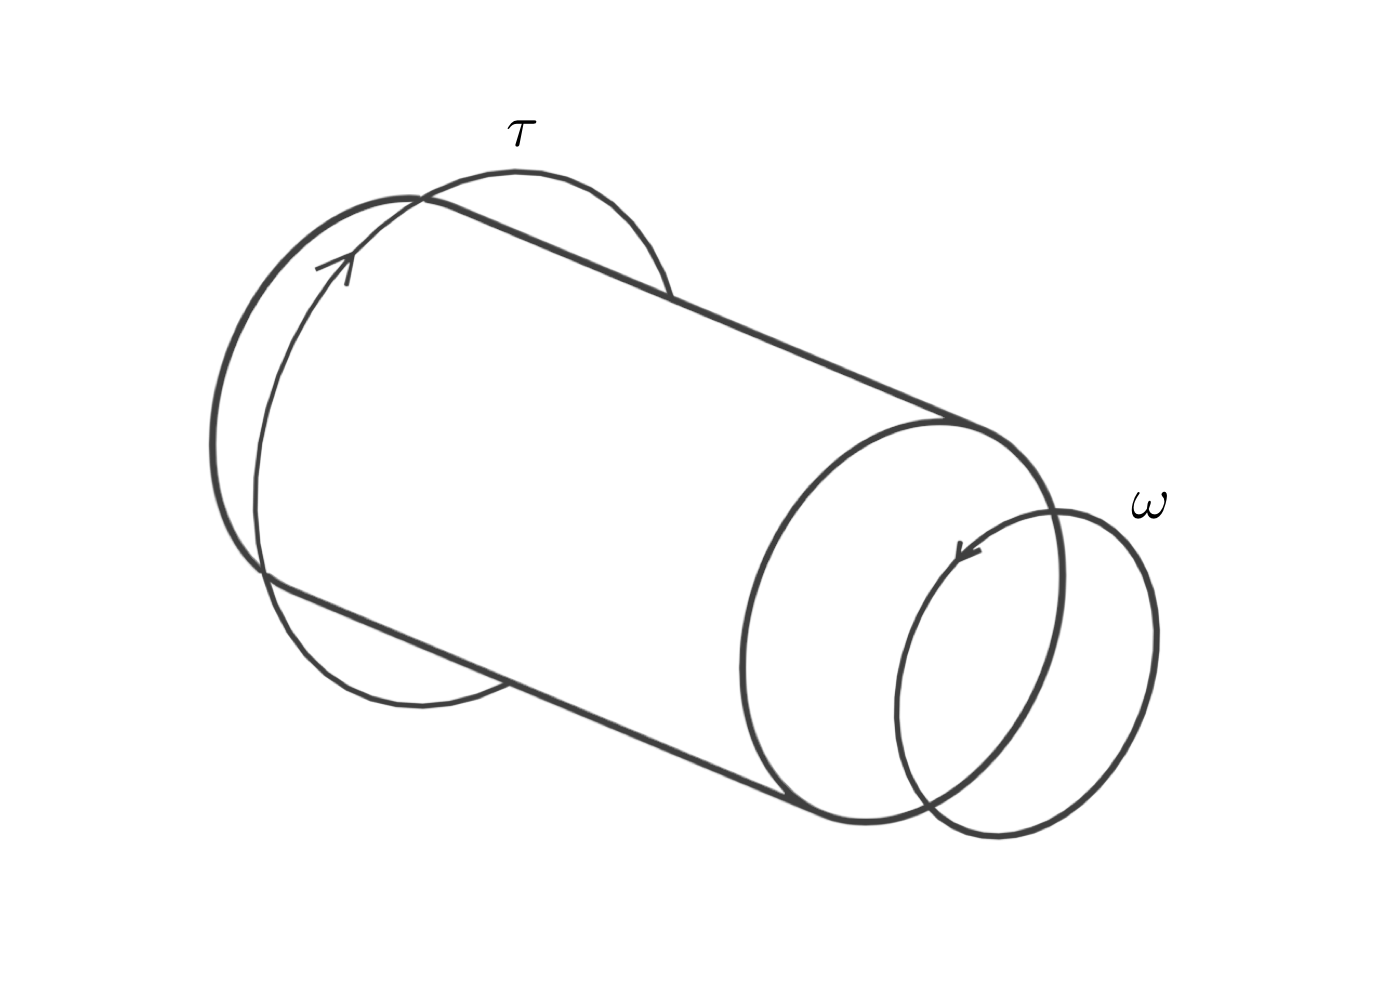
\includegraphics[width=\linewidth]{assets/20260725-1.png}
\end{minipage}
\end{center}

Assume the rotor has moment of inertia $I$ and no external torque acts on it.

\begin{questions}
  \item \textbf{A naive controller.}
        Dr.\ Wen first chooses the sensor
        \[
            S(\omega)=\omega-\omega_0 ,
        \]
        where $\omega_0>0$ is a constant.  Using the control law above and Newton's Second Law in rotational form, show that for any constant voltage $U$, the rotor converges to a steady angular velocity, and determine the steady-state value.

  \item \textbf{The improved controller.}
        Dr.\ Wen replaces the sensor with
        \[
            S(\omega)=\ln\left(\frac{\omega}{\omega_0}\right).
        \]
        He claims that logarithms are more suitable for controlling multiplicative quantities.  Show that the motor converges again, and determine the steady-state relation between $\omega$ and $U$.
\end{questions}

\end{problem}

\begin{solution}{20260725}

\subsection*{Q1. A naive controller}

\begin{align*}
    \tau &= I \dot \omega & &\text{(Newton)} \\
    k E &= I \dot \omega & &\text{(response)} \\
    k(\alpha U - S(\omega)) &= I \dot \omega & &\text{(instantiate)} \\
    k(\alpha U - \omega + \omega_0) &= I \dot \omega & &\text{(naive sensor)} \\
    \int \frac{\mathrm d \omega}{\alpha U + \omega_0 - \omega} &= \int \frac{k}{I}\;\mathrm d t & &\text{(separate)} \\
    -\ln|\alpha U + \omega_0 - \omega| &= \frac{k}{I}t + C & &\text{(integrate)} \\
    \omega(t) &= \alpha U + \omega_0 - C'e^{-kt/I} & &\text{(solve)}
\end{align*}
Taking the limit,
\[
    \omega_{\mathrm{ss}} = \lim_{t\to\infty}\omega(t) = \boxed{\alpha U + \omega_0}.
\]

\subsection*{Q2. The improved controller}

Instantiate the control law:
\[
    I \dot \omega = k\!\left(\alpha U - \ln\frac{\omega}{\omega_0}\right).
\]
At steady state $\dot\omega=0$, so
\[
    k\!\left(\alpha U - \ln\frac{\omega_{\mathrm{ss}}}{\omega_0}\right) = 0
    \;\Longrightarrow\;
    \ln\frac{\omega_{\mathrm{ss}}}{\omega_0} = \alpha U
    \;\Longrightarrow\;
    \omega_{\mathrm{ss}} = \omega_0 e^{\alpha U}.
\]
Convergence: rewrite the dynamics as
\[
    \dot\omega = \frac{k}{I}\!\left(\alpha U - \ln\frac{\omega}{\omega_0}\right).
\]
If $\omega>\omega_{\mathrm{ss}}$ then $\ln(\omega/\omega_0)>\alpha U$, so $\dot\omega<0$ (decelerates).  If $\omega<\omega_{\mathrm{ss}}$ then $\ln(\omega/\omega_0)<\alpha U$, so $\dot\omega>0$ (accelerates).  In both cases the rotor is driven toward $\omega_{\mathrm{ss}}$, hence
\[
    \boxed{\lim_{t\to\infty}\omega(t) = \omega_0 e^{\alpha U}}.
\]

\end{solution}

\input qpd-end
